\documentclass[a4paper, titlepage]{ltjsreport} % standard class
\usepackage{fontspec}
\usepackage{luatexja-fontspec}
\usepackage[Haranoaji]{luatexja-preset}
\usepackage[version=4]{mhchem} % chemical formula
\usepackage{siunitx} % e.g. \SI{1}{cm}  
\usepackage{graphicx} % figure
\graphicspath{{./fig/import/}} % path of figure
\usepackage{amsmath}
\usepackage{amssymb} % if you load unicode-math package, you should not load this package.
\usepackage{bxtexlogo} % logo such as "\pdftex"
\bxtexlogoimport{*,**} % setting for bxtexlogo
\usepackage[example]{cnltx} % for TeX/LaTeX command

\usepackage[unicode, hidelinks, draft = false, pdfusetitle]{hyperref} % hyperlink

\hypersetup{% setting hyperref
  bookmarksnumbered=true,
  bookmarksopen=true,
  bookmarkstype=toc,
  pdfborder={0 0 0},
  colorlinks = false
}

\usepackage{footnotebackref}
\usepackage{cleveref} % cross reference
% \crefname{type}{singlur form}{plural form}
\crefname{equation}{式}{式}
\crefname{table}{表}{表}
\crefname{figure}{図}{図}
\crefformat{chapter}{第#2#1#3章}
\crefname{section}{節}{節}
\usepackage{booktabs}
\usepackage{sty/titlelayout} % fix \maketitle
\subject{修士論文}
\title{学位論文用{\LaTeX}テンプレート}
\author{野口匠}
\affiliation{高知工科大学大学院 河野研究室}
\date{\today}

\usepackage{xparse}

\usepackage[%
backend = biber,%
articletitle = false,%
url = false,%
doi = false,%
eprint = false,%
isbn = false,%
sortcites = true, % \cite{paper1, paper2, paper3} -> [1-3]
style = phys%
]{biblatex} % use "biblatex"
\addbibresource{reference/reference.bib}
%
\DeclareFieldFormat[article]{journaltitle}{\mkbibemph{#1}}
%
% replace journal name with its abbreviations
%
\DeclareSourcemap{
    \maps[datatype=bibtex, overwrite=true]{
        \map{
            \step[fieldsource=Journal,
                match=\regexp{Applied\sPhysics\sLetters},
                replace={Appl. Phys. Lett.}]
            \step[fieldsource=journal,
                match=\regexp{Journal\sof\sNanoscience\sand\sNanotechnology},
                replace={J. Nanosci. Nanotechnol.}]
            \step[fieldsource=journal,
                match=\regexp{Japanese\sJournal\sof\sApplied\sPhysics},
                replace={Jpn. J. Appl. Phys.}]
        }
    }
}

\begin{document}

\maketitle

\tableofcontents

\begin{abstract}
    この研究はすごい.
\end{abstract}

\chapter{Introduction} \label{chap:introduction}

\section{Background and purpose} \label{sec:chap::introduction_background}

{\TeX}/{\LaTeX} is widely used when documents such as reports or theses is written.
This is because {\TeX}/{\LaTeX} is a system for markup language
so that users can easily separate
structure and appearance of documents.
In most laboratory, some {\LaTeX} templates is shared so that students can focus only on
the logical structure of these theses.

However, researchers is always not familiar with {\TeX}/{\LaTeX}.
This is why the templates is often too old.
Thus some error or bad appearance can occur in modern {\TeX}/{\LaTeX} system.

This template provides modern {\LaTeX} environment for theses using {\pdfLaTeX}.

\section{Feature} \label{sec:chap::introduction_feature}

Note that this template employs
\begin{itemize}
    \item \cls*{scrreprt} as document class,
    \item \verbcode{llmk} as build tool.
\end{itemize}

\section{Equation and Cross Reference} \label{sec:chap::introduction_equation}

If you want to typeset \emph{inline} mathematical formula,
you should write like \verbcode{$ formula $}
such as $x + y$ or $a = b$.

If you want to typeset single \emph{display} mathematical formula, you should write a pair of
\verbcode{\[} and \verbcode{\]} or \verbcode{equation} environment.
For example, if you use the pair of \verbcode{\[} and \verbcode{\]},
it will be
\[
    y = ax^2 + bx + c \text{,}
\]
if you use \env*{equation} environment%
\footnote{%
    If you use \env*{equation*} environment,
    the equation will not be put a number.
    Generally, if you use some environment for equation with stared,
    the equations will not be put any number.
}%
, it will be
\begin{equation}
    y = \sin x + 2 (x + y) + \sqrt{x} + \sqrt[3]{x} \text{.}
    \label{eq:chap::introduction_sec::background_sinparensqrt}
\end{equation}

The below equation is put a number and you can label by using a \cs*{label} command.
Then, you can reference a \cs*{ref} command
such as \ref{eq:chap::introduction_sec::background_sinparensqrt}.
You can refer to not only equation by \cs*{ref} command,
you can also refer to chapter, section, figure, table {\etc}
For equation, you can use a \cs*{eqref} command such as
\eqref{eq:chap::introduction_sec::background_sinparensqrt}.
However, I recommend \cs*{cref} or \cs*{Cref} command provided by \pkg*{cleveref} package,
where the \cs*{Cref} is used for the initial of sentences.

If you want to typeset multiline display mathematical formula,
you should use appropriate environment provided by \pkg*{amsmath} package.
Normally, you should use \env*{align} environment like
\begin{align}
    \sin^2 x + \cos^2 x = 1,
    \label{eq:chap::introduction_sec::equation_sincos} \\
    \tan x = \frac{\sin x}{\cos x} \text{.}
    \label{eq:chap::introduction_sec::equation_tan}
\end{align}
You can use a character ``\verbcode{&}'' into \env*{align} environment
and it makes the equations sorted:
\begin{align*}
    \cos 2x & = \cos^2 x - \sin^2 x     \\
            & = 1 - 2 \sin^2 x          \\
            & = 2 \cos^2 x - 1 \text{.}
\end{align*}

\section{Table and Figure} \label{sec:chap::introduction_table}

If you want to typeset table, you should write like this:
\begin{table}[htbp]
    \centering
    \caption{Production method of \ce{SiC} nanowire}
    \label{tab:chap::introduction_sec::introduction_sicnanowire}
    \begin{tabular}{ccc}
        \toprule
        Source    & Substrate & Catalyst \\ \midrule
        Saccharin & \ce{Si}   & \ce{Fe}  \\
        Saccharin & \ce{Si}   & \ce{Ni}  \\
        \bottomrule
    \end{tabular}
\end{table}

If you want to include figure, you should write like this:
\begin{figure}[htbp]
    \centering
    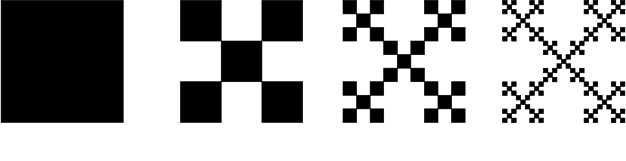
\includegraphics[width=100mm]{vicsek.pdf}
    \caption{The first, second, third part of construction of Vicsek snowflake.}
    \label{fig:chap::introduction_sec::introduction_vicseksnowflake}
\end{figure}

You can also refer to table and figure by a \cs*{cref} command
like \cref{tab:chap::introduction_sec::introduction_sicnanowire}
or \cref{fig:chap::introduction_sec::introduction_vicseksnowflake}.

\section{Citation} \label{sec:chap::introduction_citation}

You can cite other publications by \cs*{cite} command like
\cite{10.1093/jmicro/dfaa015}.
You can also cite multiple publications by single \cs*{cite} command
like \cite{10.1093/jmicro/dfaa015,Hayashi:2020:1533-4880:3038,Ishida_2019,doi:10.1063/1.4894003}.
Before citation, you must note the data of the publications
in \verbcode{.bib} file.
Then, you should include the \verbcode{.bib} file
by a \cs*{addbibresource} command provided by \pkg*{biblatex} package.
In this template, the ``phys'' style is employed.

If you use \pkg*{biblatex} package, you should build the document as follows:
\begin{itemize}
    \item Run ``\verbcode{pdflatex thesis}'' on your terminal,
    \item run ``\verbcode{biber thesis}'' on your terminal,
    \item run ``\verbcode{pdflatex thesis}'' on your terminal.
\end{itemize}



\section{Auto Build} \label{sec:chap::introduction_autobuild}

You can automate above procedure by \verbcode{llmk}.
If you want to use \verbcode{llmk},
you should clone the script from Github page of \verbcode{llmk}%
\footnote{\url{https://github.com/wtsnjp/llmk}},
and its document are there.


\printbibliography[title=参考文献, heading=bibintoc]
\end{document}